\textcolor{red}{Precisa dizer qual o papel da luz ultra-violeta primeiro. Não lembro de te visto escrito no texto ainda.}

\textcolor{blue}{A incidência de luz ultravioleta sob o feixe de nanopartículas fornece energia para o mesmo. Desta forma um número maior de \textit{clusters} presentes no feixe poderão apresentar um maior grau de ionização; por consequência maior corrente e também um aparecimento mais frequênte de \textit{clusters} com \textit{"números mágicos"}.}

Para realizar experimentos com incidência de luz ultra violeta foi preciso montar um sistema de iluminação, que consiste em inserir um LED do UV, modelo \textit{UVTOP240 TO39} produzido pela \textit{Roithner Lasertechnik GmbH}, na fonte de agregados. Para isto foi instalado um passante de tensão para que o LED fique em dentro da máquina. Além disso, um sistema de alimentação com controle de corrente foi montado utilizando uma fonte de tensão.

O LED é baseado em AlGaN (Alumínio, Gálio e Nitrogênio), com um pico típico de comprimento de onda de $245 nm$ e potência de saída óptica de $30-70 \mu W$. Seu encapsulamento é metálico e hermeticamente fechado, com configuração de lente de vidro plano. Uma foto desse diodo pode ser vista na Figura \ref{fig:foto_led}.

\begin{figure}
  \centering
  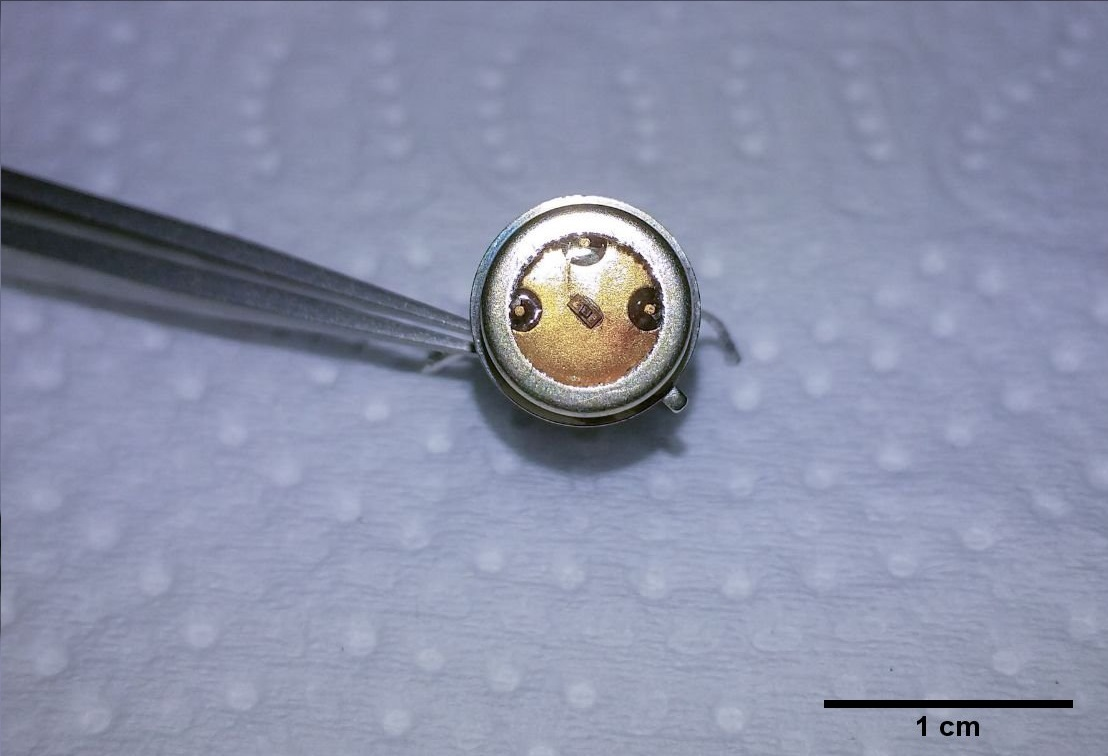
\includegraphics[width=0.7\textwidth]{images/foca/led_scale}
  \caption{ Foto do LED do UV, modelo UVTOP240 TO39, utilizado para ionização das nanopartículas.  }
  \label{fig:foto_led}
\end{figure}


Foi escolhido posicionar o LED entre a saída da câmara de agregação e a primeira lente eletrostática, como podemos ver na Figura \ref{fig:led_montagem}. Os testes do aparato consistem na aquisição da corrente de agregados produzidos e do seu espectro de massa sem o uso do LED e, posteriormente, com o LED. Com isso foi avaliado o possível aumento de ionização, como a incidência de luz afeta o espectro de massa do sistema de agregação e possíveis ajustes nos valores da tensões das lentes eletrostáticas.
Assim, foram realizados experimentos com incidência de luz ultra violeta (UV), induzindo a sua ionização, e foram comparados os espectros de abundância obtidos com e sem o uso da luz UV. 



\begin{figure}
  \centering
  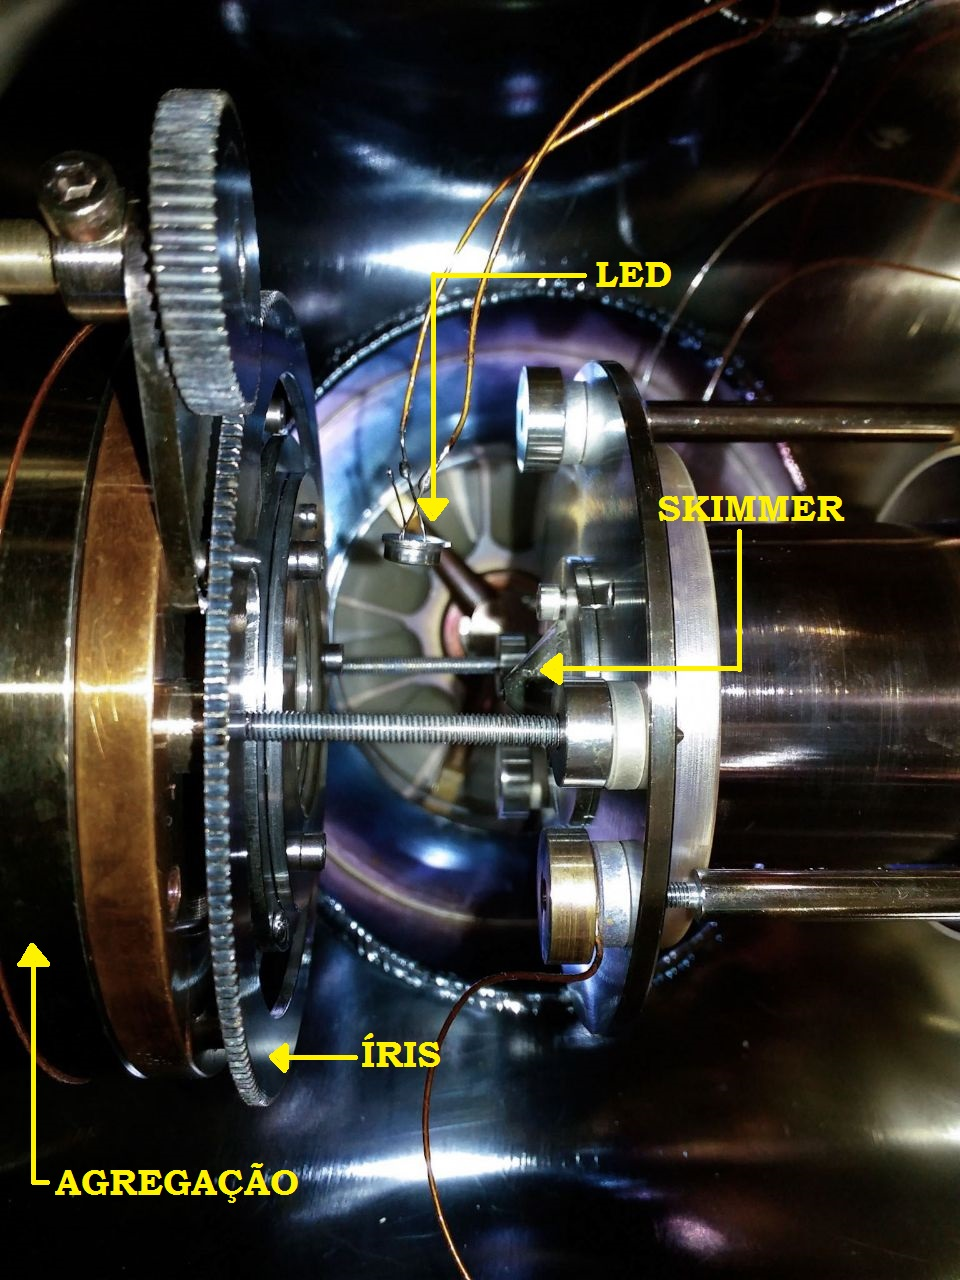
\includegraphics[width=0.5\textwidth]{images/foca/led_montagem}
  \caption{Foto do posicionamento do LED, localizado entre a câmara de deposição e a primeira lente eletrostática, Skimmer. Também está indicado a íris, peça que controla a pressão na câmara de agregação.}
  \label{fig:led_montagem}
\end{figure}
